% Chapter nc_route: a route to the Riemann Hypothesis. Volume I, before the conclusions.
% Numbers are computed by code/nc_route_*.py and the scripts of the chapter on Cauchy mixtures; those of the runs section are certified where it says so.

This chapter assembles the results of the volume into one route to the Riemann Hypothesis, says which steps of it are theorems, and states the one step that is missing. It does not prove RH. Its purpose is to make the missing step as small and as precise as the book allows, and to compare the route with the one setting in which the Riemann Hypothesis is a theorem, curves over finite fields, where the same step is supplied by geometry.

The route is the descent in level of Section~\ref{ov1:sec:path}, read in the language of Lee and Yang. Its target has six equivalent forms, each proved equivalent to RH elsewhere in the book (Section~\ref{route:sec:target}). Its top, the level one or the coupling $\frac12$, is a theorem in (T1), (T2), (T3), (T5) and (T6) (Section~\ref{route:sec:top}). The step from the top to the critical line passes three filters that rule out whole classes of argument (Section~\ref{route:sec:filters}). For curves the step is Hasse's and Weil's positivity, and a computation shows how it decides each curve through finite sections (Section~\ref{route:sec:curves}), and the runs of Section~\ref{route:sec:runs} carry the same finite sections for $\zeta$, for the Davenport and Heilbronn function and for curves of genus up to $3$ much further than the pilot. What is missing for $\zeta$ is a positive form built from the primes whose values are those of Weil's functional (Section~\ref{route:sec:missing}). The chapter ends with a work plan of problems ordered by how much of the gap each would close.

\section{The target in six forms}\label{route:sec:target}

Let $L(s)=\xi(\frac12+s)/\xi(\frac12)$, the moment generating function of the P\'olya law $p$, and let $u_\theta(v)=\pi^{-1}\re(\xi'/\xi)(\theta+iv)$ be the Thorin density at level $\theta$. The following are equivalent to RH.

\begin{enumerate}
\item[(T1)] Descent in level. For every $\alpha\in(\frac12,1)$ and $t\ne0$, $v_\alpha(t)>b_\alpha$; the minimum of the Thorin density at the origin persists from level one down to $\frac12$ (Theorem~\ref{thm:dbeta:minall}).
\item[(T2)] Deconvolution. The level one density is the Cauchy smoothing of a positive measure at the full width $\frac12$; equivalently the backward Cauchy flow runs from level one to the line through positive measures (Theorem~\ref{tf:thm:deconv}).
\item[(T3)] Cauchy mixture of one width. At one basepoint $\alpha\ge1$, $v_\alpha/\pi=P_{\alpha-1/2}*\nu$ with $\nu\ge0$ (Theorem~\ref{cm:thm:single}).
\item[(T4)] Weil positivity. $\sum_\rho\widehat h(t_\rho)\ge0$ for $h=g*\tilde g$, $g$ smooth of compact support; it is the canonical measure of the sine squared lemma undamped to the line (Theorem~\ref{cm:thm:weil}, \cite{Weil52}).
\item[(T5)] Ferromagnetism. The P\'olya law is ferromagnetic, its characteristic function in the Laguerre P\'olya class (Chapter~\ref{chap:ferro}).
\item[(T6)] Two spin Lee and Yang property, or monotonicity. The P\'olya spin coupled to one Ising spin is a Lee and Yang ferromagnet at every coupling $w>0$; equivalently $|\xi(\sigma+it)|$ is nondecreasing in $\sigma\ge\frac12$ for every $t$ (Theorem~\ref{cm:thm:mono}, \cite{SD10}).
\end{enumerate}

Each form has a parameter that measures how far from the line the statement is known: the level $\theta$ in (T1) and (T2), the width in (T3), the support of the test function in (T4), the tilt $w$ of the law $\cosh(wx)\,p$ in (T5), and the coupling $w$ in (T6). In (T1), (T2), (T3), (T5) and (T6) the parameter at which the statement holds unconditionally corresponds to the line $\re s=1$, and in (T2), (T3) and (T6) lowering it is equivalent to a zero free half plane (Theorem~\ref{cx:thm:positivity}, Corollary~\ref{cm:cor:pair}). The six forms are one statement in six coordinates.

\section{The path, and what is proved at the top}\label{route:sec:top}\label{ch:path}\label{sec:ch25:path}

The path is a programme with its gap identified, not a proof.

Figure~\ref{fig:ch25:path} and Table~\ref{tab:ch25:path} set out the path along the basepoint, and then the statements that hold with no hypothesis at the top of the descent in each of the forms of Section~\ref{route:sec:target}.

\begin{figure}[htbp]
\centering
\begin{tikzpicture}[node distance=0.55cm and 0.5cm, every node/.style={font=\small}, box/.style={draw, rounded corners, align=center, minimum width=3.4cm, minimum height=0.9cm, inner sep=3pt}, arr/.style={->, thick}]
\node[box, fill=blue!8] (primes) {primes, gamma factor,\\ pole (L\'evy side)};
\node[box, fill=orange!12, right=1.3cm of primes] (lemma) {sine squared lemma\\ (positive kernel)};
\node[box, fill=blue!8, right=1.3cm of lemma] (zeros) {zeros as atoms\\ (Thorin side)};
\node[box, fill=green!10, below=of lemma] (rho) {Thorin density $\rho_\varepsilon$\\ at basepoint $\frac12+\varepsilon$};
\node[box, fill=yellow!15, below=0.8cm of rho] (amid) {$\frac12<\alpha<1$: GGC iff\\ no zeros right of $\alpha$;\\ almost GGC};
\node[box, fill=green!10, left=0.8cm of amid] (a1) {$\alpha\ge1$: GGC\\ proved (Chapters~\ref{chap:basepoint} to \ref{chap:almost})};
\node[box, fill=red!10, right=0.8cm of amid] (acentre) {$\alpha\downarrow\frac12$: GGC\\ iff RH};
\node[box, fill=gray!10, below=0.7cm of amid] (need) {needed: $T_\alpha$ a GGC at one $\alpha<\frac78$,\\ then uniformly in $\alpha$ and height};
\draw[arr] (primes) -- (lemma); \draw[arr] (lemma) -- (zeros);
\draw[arr] (lemma) -- (rho); \draw[arr] (zeros) |- (rho);
\draw[arr] (rho) -- (a1); \draw[arr] (rho) -- (amid); \draw[arr] (rho) -- (acentre);
\draw[arr] (a1) -- (amid); \draw[arr] (amid) -- (acentre);
\draw[arr] (amid) -- (need);
\end{tikzpicture}
\caption{The Thorin path to RH. The sine squared lemma connects the arithmetic to the Thorin density. The programme must carry the GGC property across the strip.}
\label{fig:ch25:path}
\end{figure}

\begin{longtable}{p{0.05\textwidth}p{0.55\textwidth}p{0.3\textwidth}}
\caption{The path, step by step.}\label{tab:ch25:path}\\
\toprule
step & statement & status\\
\midrule
\endfirsthead
\toprule
step & statement & status\\
\midrule
\endhead
1 & The clock is infinitely divisible and self decomposable; the heat trace is positive and decreasing & proved (Theorem~\ref{thm:ch12:idsd}, which is Theorem A of \cite{P26}), with the verification of RH below height $1000$ as input\\
2 & The heat trace is log convex, its leading Hankel blocks of size up to $3\times10^7$ are positive definite, derivative signs hold to order $1.16\times10^{25}$ & proved, with verification height as input\\
3 & The reciprocal at basepoint $\alpha\ge1$ is a GGC with Poisson Thorin density (a positive Cauchy mixture at level one, with its global minimum at the origin, Proposition~\ref{bp:prop:v1min}; its atoms would be zeros on $\re s=1$, of which there are none), and at $\alpha=1$ its L\'evy form, hitting time, scale mixture and completeness are explicit; for every $\alpha>\frac12$ the shifted clock $T_\alpha$ exists and is an almost GGC & proved (Theorems~\ref{thm:poisson}, \ref{bp:thm:alpha} and \ref{ag:thm:almost}; Chapters~\ref{chap:basepoint} to \ref{chap:almost}), with the verification of RH below height $1000$ as input to Theorem~\ref{bp:thm:alpha}\\
4 & The normalised reciprocal zeta function is infinitely divisible; the canonical function of the floor of the reciprocal Xi function is an arithmetic part plus a completely monotone archimedean part, and RH is the complete monotonicity of the sum & proved (Chapters~\ref{chap:rzeta} and \ref{chap:rzid})\\
5 & The Thorin density is computable at every resolution, with an explicit bound for each source of error, and is positive at every sample point of every window computed; the runs do not yet add these bounds to the ball radii (Section~\ref{st:sec:wp2}) & computed (Chapters~\ref{chap:evaluation} to \ref{chap:heat})\\
6 & Zero density $\nu(\frac12+\varepsilon,200)=0$ for every computed $\varepsilon$, down to $\varepsilon=0.005$ & computed (Section~\ref{ch:turing})\\
7 & For some $\alpha<1$ the shifted clock $T_\alpha$ is a GGC, equivalently, the half plane $\re s>\alpha$ is zero free (Theorem~\ref{thm:poisson}); then for every $\alpha'>\alpha$ the measure $U_{\alpha'}$ is the Thorin measure of $T_{\alpha'}$ and is positive at all heights & announced for $\alpha=\frac78$ in October 2026, with a formal proof in Lean, not yet refereed (Section~\ref{sec:ch25:open}); open for every $\alpha<\frac78$\\
8 & Positivity of $U_\alpha$ for every $\alpha>\frac12$ (Lagarias), equivalently the Thorin condition & open; equivalent to RH\\
9 & The hyperbolic cosine tilted law $\cosh(wx)\,p$ is ferromagnetic for every $w\ge\frac12$, and the P\'olya spin coupled to an Ising spin is a Lee and Yang ferromagnet at every coupling $w\ge\frac12$ & proved (Theorem~\ref{cm:thm:tilt}, Corollary~\ref{cm:cor:pair})\\
10 & Ferromagnetic couplings of symmetric P\'olya spins never move the zeros of the partition function out of the strip of a single spin & proved (Theorem~\ref{cm:thm:stripXi}), by Lieb and Sokal's Proposition 2.2 as restated by Kozitsky\\
11 & The two spin system built from the truncated Euler product $E_N$ has its Lee and Yang threshold exactly at the coupling $\frac12$ & proved (Proposition~\ref{cm:prop:euler})\\
12 & At every level $\theta\in(\frac12,1)$ the Thorin measure is positive up to a fraction $O(T^{-(\theta-1/2)/4})$ of its mass on $(0,T]$ & proved (Theorem~\ref{cf:thm:negmass})\\
13 & The P\'olya law lies within total variation $1.932\times10^{-6}$ of a law shown to be ferromagnetic & proved, with a computer assisted positivity proof (Proposition~\ref{fm:prop:tvcert})\\
14 & The descent is certified in windows: Weil positivity to finite support lengths, and the positivity of $u_{3/4}$ and $u_{7/8}$ on $[0,1420]$ together with the zero count $N(T^*)=1000$ & computed (Chapters~\ref{chap:wt} and~\ref{chap:cx}), extended in Section~\ref{route:sec:runs}\\
\bottomrule
\end{longtable}

Section~\ref{bp:sec:compare} and Table~\ref{sb:tab:results} compare the constructions at and below the basepoint one: at the basepoint they are unconditional and explicit, except for the Krein string of Corollary~\ref{bp:cor:kent} (RH and simple zeros) and the Wald defect of Lemma~\ref{bp:lem:wald} (observed, not proved, for the computed boundary); below it each holds, up to a boundary case, exactly when no zero lies to the right of $\alpha$.

Step 11 is the reason the top sits where it does. The Euler product converges absolutely only on $\re s>1$, and its symmetrised truncation $E_N$ of Proposition~\ref{cm:prop:euler} has its zeros exactly on $\re s=0$ and $\re s=1$; heuristically, the unconditional results stop at the coupling $\frac12$ because that is as far as finite products of Euler factors reach.

\begin{remark}[The partial Euler products in the strip]\label{route:rem:partial}
Absolute convergence is not the end of the story, because the partial products fail to converge in the strip for a reason that is exactly the pole. Put $P_X(s)=\prod_{p\le X}(1-p^{-s})$ and $\mathrm{Li}(X^{1-s})=-E_1((s-1)\log X)$. (i) For $\frac12<\re s<1$ and $\im s\ne0$ the products $P_X(s)$ do not converge, with no hypothesis on the zeros. (ii) The Riemann Hypothesis holds if and only if $P_X(s)\exp\{\mathrm{Li}(X^{1-s})\}\to1/\zeta(s)$ locally uniformly on $\{\re s>\frac12,\ \im s>0\}$. Status: proved, from the prime number theorem with the classical error term and from $\pi(x)=\mathrm{li}(x)+O(x^{1/2}\log x)$ under RH \cite{Titchmarsh}. The behaviour of the partial products in the right half of the strip, with a modified logarithmic integral as the compensating term, is studied by Akatsuka \cite{Akatsuka17}. For (i), $\log|P_X(s)|=-\re\sum_{p\le X}p^{-s}+c_X$ with $c_X$ convergent for $\re s>\frac12$, and partial summation gives $\sum_{p\le X}p^{-s}=X^{1-s}/((1-s)\log X)\,(1+o(1))$, whose real part is unbounded above and below since the phase of $X^{-i\,\im s}$ rotates, so $|P_X(s)|$ is unbounded. For (ii), if RH holds, partial summation against $\pi=\mathrm{li}+O(x^{1/2}\log x)$ shows that $\sum_{p\le X}p^{-s}-\mathrm{Li}(X^{1-s})$ converges locally uniformly for $\re s>\frac12$, so the limit is analytic there and equals $1/\zeta$ for $\re s>1$, hence everywhere by continuation; conversely a locally uniform analytic limit equal to $1/\zeta$ on $\re s>1$ continues $1/\zeta$, so $\zeta$ has no zero with $\re s>\frac12$. Computed with the primes up to $2\times10^8$: at $s=0.6+2i$ the corrected product is $1.4443+0.9962i$ against $1/\zeta=1.4422+0.9932i$, while $|P_X|$ itself is $8\times10^{11}$ at $X=10^8$ and $1.5\times10^{-15}$ at $X=2\times10^8$. So the pole term alone blocks the product, and removing it leaves a function whose singularities in the strip are exactly the zeros (heuristic: by (ii) the corrected product converges in the strip only under the Riemann Hypothesis). This is the sharp form of the paragraph above, and it is not the M\"obius series of Titchmarsh, which has no pole to fight. The statement is from an unrefereed note of Polson (November 2026), where the claim that the products converge in the strip under RH is false; it is corrected here.
\end{remark}

\section{Three filters on the missing step}\label{route:sec:filters}

Section~\ref{ov1:sec:path} states three constraints. Read as filters on a candidate for the missing step, they say the following.

\begin{enumerate}
\item The step cannot be a finite computation, nor any argument that sees only finitely many zeros (Theorem~\ref{thm:ch13:perturb}). For curves the corresponding statement is false, since finitely many point counts determine the zeta function; this is the first place where the analogy breaks.
\item The step must use the Euler product, because the Davenport and Heilbronn function shares the functional equation, the Cauchy structure and the positivity of the trace, and has zeros off the line (Theorem~\ref{bsy:thm:dhid}).
\item The step must not rest on a property preserved by Gaussian damping (Proposition~\ref{ki:prop:obstruction}). In Lee and Yang terms, every general theorem available, from Lee and Yang to Newman and to Lieb and Sokal, preserves the property when ferromagnetic interactions are added; RH asks for one to be removed, and $\Lambda\ge0$ \cite{RodgersTao} says that the self interaction of the de Bruijn Newman flow cannot be made negative.
\end{enumerate}

The first filter excludes the computations of the books as proofs, while keeping them as refutations. The third excludes the strip Lee and Yang theorem of step 10 above as a proof: it adds couplings. What survives the three filters is a positivity statement, for all heights at once, that uses the primes.

\section{The benchmark: curves over finite fields}\label{route:sec:curves}

For an elliptic curve the completed zeta function is a Frobenius spin, and the Hasse bound is its ferromagnetism (Proposition~\ref{cm:prop:frob}). Hasse's proof supplies the positivity from the degrees of isogenies, and in the language of (T4) it is Weil positivity on two point test functions. For a curve of genus $g$ the same structure has $g$ Frobenius spins, one for each pair of eigenvalues $\alpha_j,\bar\alpha_j$, and the analogue of Weil's functional is a Toeplitz form.

\begin{proposition}\label{route:prop:toeplitz}
Let $C$ be a smooth, projective, geometrically irreducible curve of genus $g$ over $\mathbb F_q$ with $N_n$ points over $\mathbb F_{q^n}$, and put $s_0=2g$ and $s_n=s_{-n}=(q^n+1-N_n)/q^{n/2}=\sum_{j=1}^{2g}\alpha_j^n/q^{n/2}$ for $n\ge1$, the $\alpha_j$ being the $2g$ Frobenius eigenvalues. The Riemann Hypothesis for $C$, $|\alpha_j|=\sqrt q$ for every $j$, holds if and only if the Toeplitz matrices $(s_{k-l})_{0\le k,l<n}$ are positive semidefinite for every $n$.
\end{proposition}

\begin{proof}
If $|\alpha_j|=\sqrt q$, write $\alpha_j=\sqrt q\,e^{i\theta_j}$; then $s_n=\sum_{j=1}^{2g}e^{in\theta_j}$ are the Fourier coefficients of the positive measure $\sum_{j=1}^{2g}\delta_{\theta_j}$ on the circle, and the Toeplitz matrices are positive semidefinite. Conversely, positive semidefinite Toeplitz matrices of every size have entries bounded by $s_0$ (already the $2\times2$ principal submatrices give this), so the sequence $s_n$ is bounded; but if some $|\alpha_j|\ne\sqrt q$, the functional equation pairs $\alpha_j$ with $q/\alpha_j$, one of the two has modulus above $\sqrt q$, and $s_n$ is unbounded.
\end{proof}

The finite sections of the Toeplitz form play the part of the windows of Weil positivity for $\zeta$. For the curve $y^2=x^5+x+1$ of genus $2$ we counted points over $\mathbb F_p$ and $\mathbb F_{p^2}$ for $p=11,13,17,19,29,31$ (the curve is singular modulo $3$, $7$ and $23$, where the computation does not apply), which determines the numerator $1+c_1T+c_2T^2+pc_1T^3+p^2T^4$ of the zeta function: for every one of these primes the four Frobenius eigenvalues have modulus $\sqrt p$ to machine precision, and the Toeplitz sections of sizes $2$ to $40$ are positive semidefinite, of rank $4$ from size $4$ on. A fake numerator with the same $c_1$ and $c_2$ moved outside the region the Riemann Hypothesis allows, $c_2=29$ or $c_2=-26$ at $p=13$, has eigenvalue moduli between $0.80\sqrt p$ and $1.26\sqrt p$, or $0.69\sqrt p$ and $1.46\sqrt p$, and its Toeplitz sections already fail at size $3$, with smallest eigenvalue $-2.2\times10^4$ and $-4.5\times10^6$ at size $40$ (Figure~\ref{route:fig:toeplitz}; computed).

\begin{figure}[htbp]
\centering
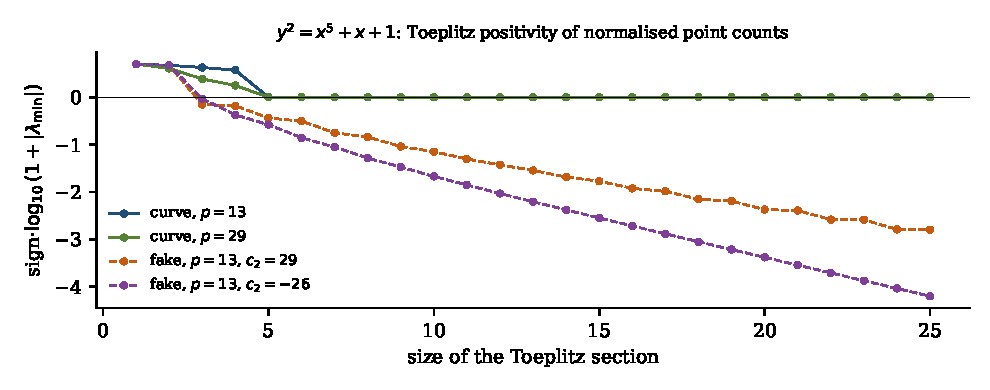
\includegraphics[width=\textwidth]{fig/route_toeplitz.pdf}
\caption{Smallest eigenvalue of the Toeplitz sections of the normalised point counts of $y^2=x^5+x+1$ at $p=13$ and $p=29$, and of two fake numerators at $p=13$, against the size of the section, on a signed logarithmic scale. The genuine curve stays at or above $0$; the two fakes plotted fail from size $3$ (computed).}
\label{route:fig:toeplitz}
\end{figure}

For a curve, three facts make the method work, and each fails for $\zeta$.

\begin{enumerate}
\item The form is positive for a reason outside the zeta function: Weil's proof uses the Castelnuovo positivity of the intersection form on $C\times C$ \cite{Weil48}.
\item The form is finite dimensional in effect: the measure has $2g$ atoms, the Toeplitz matrices have rank $2g$, and a fake numerator fails at a small size. For $\zeta$ the measure has infinitely many atoms and every finite section is passed by a perturbation whose zeros off the line lie high enough (the first filter).
\item The spins are of exponential type, so the Lee and Yang theory applies to them as they stand. For $\zeta$ the P\'olya spin has infinite type; Theorem~\ref{cm:thm:stripXi} recovers the strip statement by approximation, but no approximation can supply positivity that the limit does not have.
\end{enumerate}

\section{Finite sections for \texorpdfstring{$\zeta$}{zeta}, shrinking and bounds}\label{route:sec:round2}



\paragraph{The Hankel analogue of the Toeplitz test} For a curve the Toeplitz sections of Proposition~\ref{route:prop:toeplitz} catch the two fake numerators computed above at size $3$. For $\zeta$ the analogue is the Hankel test of Proposition~\ref{ev:prop:hankel}: with $M_j=\sum_k\gamma_k^{-2j}$, one atom for each pair of zeros, RH holds if and only if $\det[M_{i+j+1}]_{i,j<n}>0$ and $\det[M_{i+j+2}]_{i,j<n}>0$ for every order $n$. The moments are computable from $\xi$ at $\frac12$, without the zeros, so this is a test of the same kind as the curve's. We replaced the ordinates $\gamma_k,\gamma_{k+1}$ by the pair $\frac12(\gamma_k+\gamma_{k+1})\pm i\eta$ and recorded the least order at which a determinant fails (the table of Section~\ref{route:sec:runs}), with the first $220$ ordinates and the tail above them as the positive density $\frac1{2\pi}\log\frac t{2\pi}\,dt$ (computed, floating point at the precision stated).


The order needed to see a pair is about twice its index, slightly more when the pair is closer to the line; the runs of Section~\ref{route:sec:runs} give $1.7$ per index to $k=128$ (the precision of the evaluation of the moments has to grow with the order as well). Since the index of a pair at height $T$ is about $N(T)\approx\frac T{2\pi}\log\frac T{2\pi e}$, a Hankel section sees pairs off the line only up to the height where $2N(T)$ equals its order (computed). For a curve a section of size $2g=4$ catches any fake numerator with distinct roots; for $\zeta$ the size must grow without bound with the height, which is the first filter of Section~\ref{route:sec:filters} in numbers.

\paragraph{Shrinking under a Curie Weiss coupling} Problem~\ref{route:prob:shrink} has a quantitative answer when the coupling acts on the magnetisation.

\begin{proposition}\label{route:prop:cw}
Let $\chi_1,\dots,\chi_N$ be laws of Xi type in $\mathcal C_\delta$ whose densities are $O(e^{-|x|^\kappa})$ for some $\kappa>2$, and couple them with the Curie Weiss weight $e^{\frac a2S^2}$, $S=\sum_i\sigma_i$, $a\ge0$. In a common field the partition function $\E e^{\frac a2S^2+hS}$ has all its zeros in $|\re h|\le(\max(\delta^2-a,0))^{1/2}$.
\end{proposition}

\begin{proof}
The moment generating function of $S$ is $\prod_i\varphi_i$, whose zeros lie in the strip of half width $\delta$, and the density of $S$ is again $O(e^{-c|x|^\kappa})$ by convexity of $|x|^\kappa$. The weight $e^{\frac a2S^2}$ is de Bruijn's multiplier $e^{\lambda t^2}$ with $\lambda=\frac a2$, which maps a strip of half width $\Delta$ into one of half width $(\max(\Delta^2-2\lambda,0))^{1/2}$ \cite[Theorem 13]{deBruijn}, as in Proposition~\ref{fm:prop:bruijn}.
\end{proof}

The bound is sharp to first order for one spin with an isolated pair of zeros off the line: under the heat flow $\partial_a=\frac12\partial_h^2$ that the multiplier induces on the moment generating function, a zero moves with velocity $-\sum1/(r-r')$ over the other zeros $r'$, and for an isolated pair the pull of the mirror zero at distance $2\delta$ gives $\frac d{da}\delta^2=-1$ (heuristic). For $N$ copies the zero has multiplicity $N$ and the pull is $N$ times larger, $\frac d{da}\delta^2=-N$; a computation with two planted spins of strip $0.3$ found $\delta^2$ falling from $0.0900$ to $0.0860$, $0.0704$ and $0.0524$ at $a=0.002$, $0.01$ and $0.02$, that is at rate $2.0$, $2.0$ and $1.9$. The shrinking is a property of the coupled system; RH concerns the single spin, where the coupling would have to be removed.

\paragraph{Bounds along a family} There is a second proof of the Riemann Hypothesis for curves, by Stepanov and Bombieri, which goes through bounds and not through positivity of a form. It proves $|N_n-q^n-1|\le Cq^{n/2}$ for all large $n$ by constructing an auxiliary function that vanishes to high order at the rational points, the fixed points of the Frobenius map $x\mapsto x^q$, and the Riemann Hypothesis follows because bounded normalised power sums $s_n$ force $|\alpha_j|\le\sqrt q$, the argument of Proposition~\ref{route:prop:toeplitz}. The family is the tower of extensions $\mathbb F_{q^n}$. For $\zeta$ the family is the cutoff $x$, the analogue of the bound is $\psi(x)-x=O(x^{1/2}\log^2x)$, which is equivalent to RH by von Koch's theorem, and the analogue of the growth argument is the passage from the error term to the zeros through the explicit formula. In the language of this book the bound $\psi(x)-x=O(x^{\theta+\varepsilon})$ is the positivity of the Thorin density at the level $\theta$ (Section~\ref{ov1:sec:path}). What Stepanov uses and $\zeta$ lacks is the Frobenius map: a polynomial map whose fixed points are the objects counted, which lets an auxiliary function vanish at all of them with controlled degree. No such map is known on the integers, and this is the same absence, seen through bounds instead of positivity, as that of Section~\ref{route:sec:curves}.

\section{The runs}\label{route:sec:runs}

The finite sections of the previous sections were computed at pilot size. This section reports four of the five work packages that extend them (the third, the field and the two spin test, is in Section~\ref{cm:sec:gap}), each from first principles (the matrices, explicit formulae and certificates were written for this book; none of the pilot code was used). Status words: certified means ball arithmetic throughout, with a sign proved by an $LDL^T$ factorisation of balls or by a cell lemma; computed means floating point or a fit; the laws read off are computed or heuristic and prove nothing.

\paragraph{The Weil ladder} The form is the Weil functional on the $N+1$ even cosine modes of $[1/\lambda,\lambda]$, $X=\lambda^2$. It was first checked against the explicit formula: the matrix reproduces $2\sum_kF(\gamma_k)^2$ over the first $1700$ ordinates to $10^{-12}$ relative, and the pilot eigenvalues at fourteen rungs to eight digits (computed). Positivity was then certified on $266$ cells $(X,N)$, every one positive: a matrix of balls containing the exact matrix (Gauss and Legendre quadrature with a proved error bound, prime sums as finite sums of balls), and a ball $LDL^T$ with every pivot positive, with the least eigenvalue bracketed. The certified grid lies in $X\in\{2,\dots,10^4\}$ against $N\in\{8,\dots,200\}$ (not every pair), with $X$ to $10^5$ at $N\le200$ and to $10^6$ at $N\le100$ on a sparse set, $N=300$ and $N=400$ to $X=10^5$, and $N=600$ at $X=2,5,13,50,200,10^3,10^4,10^5$. These certify Weil positivity on a finite dimensional subspace, not on all functions supported in $[1/\lambda,\lambda]$. The least eigenvalue $\varepsilon$ is tiny, $9.5\times10^{-54}$ at $(13,40)$ and $9.3\times10^{-106}$ at $(1000,30)$, and falls by about $17$ and $12$ digits per doubling of $\lambda$ on $50$ to $200$ and on $200$ to $1000$ (computed). The exponential decay in $N$ seen in the pilot is a law of small $N$ only: $-\log_{10}\varepsilon/N$ falls from $3.83$ at $N=20$ to $2.28$ at $N=200$ for $X=1000$, at $X=2$ the eigenvalue saturates at $1.329\times10^{-3}$ already near $N=100$, at $X=13$ it still falls by $23$ and $10$ per cent from $N=100$ to $200$ and from $200$ to $400$, and at $X=50$ it is still falling by $37$ orders of magnitude from $N=200$ to $400$. So the decay is exponential to about $N=40$ and no law beyond is claimed. The zero of the transform nearest $\gamma_k$ is farther than $\varepsilon$, by $4$ to $18$ digits, and the distance falls like a power $1.05$ to $1.17$ of $\varepsilon$; a fit $\log_{10}\mathrm{err}_k=6.03+1.168\log_{10}\varepsilon-0.289\gamma_k+0.604\gamma_kL$ over all runs has rms residual $3.5$ digits (computed). The odd modes decouple: all $36$ cells (to $N=60$, $X=1000$) are positive (computed, sign certified).

\begin{remark}[the prime built Gaussian process is half the Weil form]\label{route:rem:gp}
Let $a>0$, $L=a/2$, $X=e^a$, and let $K(s,t)$ be the covariance on $[0,a]^2$ of the Gaussian process whose increments have the variogram of the zeros, $K(s,t)=\frac12\sum_\rho(h_s+h_t-h_{s-t})(\gamma_\rho)$ with $h_t(z)=(1-\cos zt)/z^2$. For steps $\phi_c=\sum_jc_j\mathbf 1_{[0,t_j)}$ and $f_c(x)=\phi_c(x+L)$, which are exactly the step functions on $[-L,L]$ and are dense in the form domain of the Weil functional $W_L$ and in $C_c^\infty(-L,L)$, one has $\sum_{j,k}c_jc_kK(t_j,t_k)=\frac12W_L(f_c)$ (proved). So $K$ is positive semidefinite on $[0,a]^2$ exactly when Weil positivity holds on the window of length $a$, the rung $X=e^a$ of the Weil ladder, and the criterion in that form is Suzuki's. % UNCHECKED: attribution to M. Suzuki's screw function criterion from memory, not read
A positive definite covariance matrix on a grid of step $1/40$ through $a=12$ is a statement about step functions of that step only, and adds nothing beyond the known zeros: its positivity already follows from the first $2500$ zeros, in a ball computation conditional on the verified height of the zeros, whereas under RH the margin of $W_L$ on the whole window is at most of order $10^{-888235}$ at $a=12$ (heuristic extrapolation of the law of the ladder), and the ladder above is certified only on finite dimensional subspaces. The archimedean part of the form alone first loses positivity at the window $a=0.7432$ in the odd sector and $a=0.8202$ in the even sector (computed, upper bounds converging in the fourth digit). The window results of \cite{Zhu26}, reported in Chapter~\ref{chap:zhu}, come from an unrefereed preprint whose certificates we have not rechecked, and are conditional on that status.
\end{remark}

Two replacements of $\zeta$ test the second filter of Section~\ref{route:sec:filters}. First, the Davenport and Heilbronn function, with the explicit formula derived for it (no pole term, conductor $5$, coefficients of $-f'/f$ on all integers) and validated against its zeros to $T=200$, $122$ on the line and four off it: the matrix and the zero sum agree to $10^{-15}$ relative on even modes and $2\times10^{-12}$ on odd, and the off line zeros are needed for the agreement. The form is certified positive on every cell with $N\le52$ and $X\le2000$ (at $X=30$ to $N=80$), and first certified negative at $N=56$ for $X=50,100$, at $N=60$ for $X=200,500$, and at $N=64$ for $X=1000,2000$. Two statements are supported. Proved, given the explicit formula for the Davenport and Heilbronn function: a negative section forces a zero of $f$ off the line, since the line zeros contribute $|F(\gamma)|^2\ge0$. Computed, at $X=50$ and $100$: the decomposition over the zeros of $f$, at the least eigenvector, shows the quadruple of $0.8085+85.6993i$ supplying the negative term. At $X\ge200$ the first negative cells carry no eigenvector data, and at $X=2000$, $N=60$ the decomposition does not close, so the mechanism is not shown there; nor does the size at which the form fails follow a simple rule in $\pi N/L$ ($X=30$ stays positive to $N=80$). The validation tests the off line terms only weakly: they move the test values by $10^{-14}$ to $4\times10^{-10}$, against residuals of $5\times10^{-17}$ to $2\times10^{-12}$, and it does not reach the range $N\ge52$ where that zero dominates. Second, cutting the prime sum of $\zeta$ at $Y$: the form is certified negative, with $\varepsilon$ of order one for $Y$ well below $X$ and tiny just below the last primes ($-1.1\times10^{-69}$ at $Y=983$, $X=1000$), At $N=20$ the largest $Y$ with a negative form and the smallest with a positive one are $7$ and $11$ at $X=13$, $47$ and $49$ at $X=50$, $193$ and $197$ at $X=200$, $983$ and $991$ at $X=1000$ (certified signs).

\paragraph{A pencil through two Euler products}\label{route:sec:pencil} A third replacement tests the second filter with functions that share the functional equation of $\zeta_K$ and differ from it only in multiplicativity. This paragraph is condensed from an unrefereed note of Polson (November 2026), corrected in refereeing; its numbers are the author's unless marked. Let $K=\mathbb Q(\sqrt{-15})$ have class number two, with reduced forms $Q_1=x^2+xy+4y^2$ and $Q_2=2x^2+xy+2y^2$, and let $\zeta_{Q_j}$ be the Epstein zeta functions. By genus theory $\zeta_K=\frac12(\zeta_{Q_1}+\zeta_{Q_2})=\zeta(s)L(s,\chi_{-15})$ and $L(s,\psi)=\frac12(\zeta_{Q_1}-\zeta_{Q_2})=L(s,\chi_{-3})L(s,\chi_5)$, both with Euler products and real coefficients (proved). For real $\theta$ put $F_\theta=\cos\theta\,\zeta_K+\sin\theta\,L(s,\psi)$. Every $F_\theta$ satisfies the functional equation $\Lambda_\theta(s)=(\sqrt{15}/2\pi)^s\Gamma(s)F_\theta(s)=\Lambda_\theta(1-s)$ and has a simple pole at $s=1$ with residue $2\pi\cos\theta/\sqrt{15}$ when $\cos\theta\ne0$ (proved). Write $a_n(\theta)$ for its coefficients, so $a_1=\cos\theta+\sin\theta$, $a_2=2(\cos\theta-\sin\theta)$, $a_3=\cos\theta-\sin\theta$, $a_6=2(\cos\theta+\sin\theta)$. Multiplicativity of $a_n$ requires $a_1a_6=a_2a_3$, that is $\cos\theta\sin\theta=0$, so $F_\theta$ has an Euler product exactly at $\theta\in\{0,\frac\pi2,\pi,\frac{3\pi}2\}$ (proved). At $\theta=\frac\pi4$ one has $F_\theta=\zeta_{Q_1}/\sqrt2$, an Epstein zeta function of a form of class number above one, which has zeros with $\re s>1$ by Davenport and Heilbronn \cite{DH36} (proved).

The explicit formula for $F_\theta$ has the shape of the one in Section~\ref{cp:sec:weil}, with the pole terms present when $\cos\theta\ne0$, the term $-h(0)\log\pi$ replaced by $h(0)\log(15/\pi^2)$, the archimedean term of $\zeta$ and that of an odd $L$ function in place of the single $\Gamma$ factor, and the prime sum $\sum_{n}c_n(\theta)n^{-1/2}(h(\log n)+h(-\log n))$ over $n<e^W$, where the coefficients of $-F_\theta'/F_\theta$ satisfy $a_1c_n=a_n\log n-\sum_{d\mid n,\,d<n}c_da_{n/d}$ (proved; the factor $a_1$ is needed, and $a_1\ne0$ for $0\le\theta\le\frac\pi2$). The Weil matrix of Section~\ref{cp:sec:weil} is rebuilt from this formula on a band limited basis (type $W=9$, so integers below $8104$) with $58$ centres on $[40,80]$ (computed). Its least eigenvalue is at the rounding floor, of order $10^{-10}$, at the Euler angles $\theta=0$ and $\frac\pi2$, and negative at every other sampled angle: $-0.555$, $-1.424$, $-2.089$, $-2.479$, $-2.579$, $-2.310$, $-1.471$ at $\theta=11.25^\circ$ to $78.75^\circ$ in steps of $11.25^\circ$ (computed). Positivity at the Euler angles is no finding: it follows from the generalised Riemann Hypothesis for $\zeta L(\chi_{-15})$ and $L(\chi_{-3})L(\chi_5)$ (conditional; the matrix involves every zero, while the zeros at these heights are classically on the line \cite{Rumely93}), and a direct count of sign changes finds $39$ zeros in $[43,77]$ for each of the two functions, all on the line (computed). The negative eigenvalues come with off line pairs. At the Epstein angle the matrix places pairs at $43.63\mp0.356i$, $47.53\mp0.413i$, $61.42\mp0.526i$, $64.81\mp0.229i$ and $66.78\mp0.172i$ (computed), and a root finder on $\zeta_{Q_1}$ itself gives the zeros $0.8558+43.6317i$, $0.9129+47.5332i$ and $1.0260+61.4228i$ (computed), the last the lowest zero of this function with real part above one. Weil positivity here holds on a finite dimensional span and the converse fails on a finite basis, as in Figure~\ref{cp:fig:weil}, so negativity proves that some zero is off the line but does not locate it. The fields $D=-20$ and $-24$ behave alike (nonnegative to the floor at the Euler angles, conditional as above, negative at the Epstein angle), and for $D=-23$, class number three, the real combination of the two nontrivial class characters is $L(s,\psi)$ itself, with an Euler product and a matrix nonnegative to the floor (computed, conditional as above).

The positivity set is a corner. For $D=-15$, $\lambda_{\min}(M_\theta)=-1.04\times10^{-3},-2.09\times10^{-3},-5.26\times10^{-3},-1.12\times10^{-2},-3.13\times10^{-2}$ at $\theta=0.001,0.002,0.005,0.01,0.02$ (computed): the departure from $\theta=0$ is linear with slope about $1.05$ up to $\theta=0.005$ and steeper beyond, where the next pair leaves, and the displacement of the first pair to leave grows like $\sqrt\theta$ (computed). So no tangency or plateau is seen, and positivity is lost at first order as soon as multiplicativity is. The corner is explained by a local rule, heuristic as stated. Write $F_\theta=Z_0+\tan\theta\,Z_1$ (up to a positive factor) on the line, with $Z_0,Z_1$ real, from $\zeta_K$ and $L(s,\psi)$. Let $\gamma_1<\gamma_2$ be consecutive zeros of $Z_0$ with gap $d\to0$, $t^*$ the point between them where $|Z_0|$ is largest, $|Z_1(t^*)|$ and $|Z_0''(t^*)|$ bounded below, and $Z_1$ without zero on $[\gamma_1,\gamma_2]$. If $Z_0(t^*)$ and $Z_1(t^*)$ have the same sign the zeros move apart; if the signs are opposite they merge at $\tan\theta_c\approx|Z_0(t^*)|/|Z_1(t^*)|\approx|Z_0''(t^*)|\,d^2/(8|Z_1(t^*)|)$ and leave the line as a conjugate pair with displacement $b$, $b^2\approx2(\tan\theta-\tan\theta_c)|Z_1(t^*)|/|Z_0''(t^*)|$ (heuristic; with the stated hypotheses, a nondegenerate double zero and no other zero entering, the implicit function theorem and Hurwitz's theorem would give it locally). It is the local form of the Hermite, Kakeya and Obreschkoff theorem, that all real combinations of two real polynomials with real zeros are real rooted exactly when their zeros interlace (for entire functions this needs growth conditions, as in the Hermite and Biehler theorem \cite{Levin64}), and the collision of close pairs is the mechanism of Lehmer pairs under the heat flow \cite{CSV94}. If $Z_0$ and $Z_1$ are both real rooted (the Riemann Hypothesis for both factors) and the entire function form of the theorem applies, the existence of Epstein zeros off the line \cite{DH36} would show that their zeros do not interlace (conditional). The pair $48.0031$ (a zero of $L(\chi_{-15})$) and $48.0052$ (a zero of $\zeta$) has opposite signs and predicts $\theta_c\approx2.5\times10^{-6}$ (computed), which puts the corner at the origin to working precision. What this shows is that a Weil positivity test with the gamma factors and conductor of $\zeta_K$ separates the two Euler product angles from the rest, so the form cannot be satisfied by the functional equation, the gamma factors and the pole alone, in line with the second filter. It does not show that the Euler product is the only distinction, and no claim is made that an Euler product forces positivity (open).

\paragraph{The Thorin level} The cell certificate of $u_\alpha>0$ of Chapter~\ref{chap:cx}, generalised to any level and height range, certifies that $\xi$ has no zero on $\operatorname{Re}s=\alpha$ for $|t|\le10^4$ at $\alpha=\frac78,\frac34,0.6,0.55,0.52,0.51$, and for $|t|\le10^5$ at $\alpha=\frac78,\frac34,0.6$ (no failing cell; $49\times10^6$ cells at $\frac34$ on $[10^4,10^5]$). An independent evaluation with \texttt{mpmath} agrees with the ball midpoints to $7\times10^{-17}$ relative (computed). The least certified bound of $v_\alpha=\pi u_\alpha$ on a decade is the margin.

\begin{center}\small
\begin{tabular}{rrrrr}
\toprule
$\alpha$ & $[10^2,10^3]$ & $[10^3,10^4]$ & $[10^4,10^5]$ & ratio, $[10^3,10^4]$\\
\midrule
$0.51$ & $0.0094$ & $0.0237$ & not run & $2.377$\\
$0.52$ & $0.0189$ & $0.0475$ & not run & $2.377$\\
$0.55$ & $0.0474$ & $0.118$ & not run & $2.374$\\
$0.6$ & $0.0947$ & $0.236$ & $0.402$ & $2.367$\\
$\frac34$ & $0.234$ & $0.580$ & $0.978$ & $2.321$\\
$\frac78$ & $0.347$ & $0.846$ & $1.413$ & $2.257$\\
\bottomrule
\end{tabular}
\end{center}

The ratio of the margin to $\alpha-\frac12$ is almost independent of $\alpha$ (the limit as $\alpha\downarrow\frac12$ is the sum of $(v-\gamma)^{-2}$ over the zeros at the worst point, computed, assuming the nearby zeros are on the line), so the margin is linear in $\alpha-\frac12$ uniformly in height, with a constant that grows with the height: at $\frac34$ it is $0.105$, $0.94$, $2.32$, $3.91$ on the decades from $[10,10^2]$ to $[10^4,10^5]$, which is faster than $\log T$ and about $(\log T)^2/34$ on the last decades (computed, a description of five decades). The least value is at the same $v=109.04$, $1069.30$, $10677.94$ at every level. The minimum over $v$ is at the origin: above $v^*$ (between $0.57$ and $1.6$ according to the level) every cell bound exceeds $u_\alpha(0)$ (certified), and on $(0,v^*)$ only the midpoints do (computed). The levels $0.55$ to $0.51$ above $10^4$ were not run.

\paragraph{The Hankel order} The Hankel test of Section~\ref{route:sec:round2} was rerun with all orders decided by a ball $LDL^T$ without pivoting, with $2000$ ordinates in balls of radius $10^{-719}$ and the tail above them the positive density, at $3400$ and $6800$ bits. The pilot orders of the table below, from the first $220$ ordinates, are reproduced exactly, are the same with $220$ or $2000$ ordinates and with the ordinates cut to $300$ digits, and each failing pivot is a ball below $0$ (certified for the model measure; that the zeros above $\gamma_N$ behave like the tail density is evidence, not proof). The orders continue $57,86,113,168,222$ at $k=32,48,64,96,128$ ($\eta=0.3$). They are linear in $k$ with slope about $1.7$, $n=1.717k+2.81$ (rms $0.46$), the local slope falling from $2$ to $1.69$ and no saturation to $k=128$ (computed); the width $\eta=0.1$ costs at most three orders more. The genuine moments are positive definite to order $250$ for the model measure (certified at $6800$ bits), and beyond order about $100$ the precision needed exceeds the $700$ digits first used (inferred, the $700$ digit run was not done).

\begin{center}\small
\begin{tabular}{rrcc}
\toprule
$k$ & height & order, $\eta=0.3$ & order, $\eta=0.05$\\
\midrule
$1$ & $17.58$ & $4$ & $5$\\
$2$ & $23.02$ & $6$ & $7$\\
$3$ & $27.72$ & $8$ & $9$\\
$5$ & $35.26$ & $11$ & $13$\\
$8$ & $45.67$ & $17$ & $19$\\
$12$ & $57.90$ & $24$ & $26$\\
$17$ & $70.81$ & $32$ & $34$\\
$24$ & $88.12$ & $44$ & $47$\\
\bottomrule
\end{tabular}
\end{center}

\paragraph{Curves} The Weil ladder was built for curves, by interval arithmetic on the numerator of the zeta function, with the explicit formula of Poisson summation giving the matrix $\ell[2g\,g(0)+2\sum_ms_mg(m\ell)]$ on cosine modes. Points were counted by brute force on $69$ curves of genus $1,2,3$ over every prime power $q\le49$ (the numerators are exact integers and satisfy RH to $10^{-12}$), and the ladder was run on $13$ of them (genus $1,2,3$ at $q=3,5,13,49$ and $y^2=x^5+x+1$ over $\mathbb F_{13}$) at $\tau=2L/\log q$ from $2$ to $32$ and $N$ from $2$ to $32$. Of $819$ genuine rungs, $757$ are certified positive, $6$ positive in floating point without a certificate, and $56$ are exact kernels (computed: the least eigenvalue vanishes to the working precision), the supersingular numerators $1+49T^2$ (genus $1$, $q=49$) and $1+125T^6$ (genus $3$, $q=5$), where the form is semidefinite with a nonzero kernel and strict positivity cannot hold. Of $693$ rungs of fake numerators, $626$ are certified negative; the first level at which a fake fails is $\tau=2,3,4$ for genus $1,2,3$ (at $N=2$ the genus $2$ fakes first fail at $\tau=4$; see the Toeplitz sizes $2$ and $3$ of Proposition~\ref{route:prop:toeplitz}, and for genus $3$ the product of a genuine factor and a genus $2$ fake), and the size of the failure grows like $\rho^\tau$, with $\rho$ the largest ratio $|\alpha|/\sqrt q$ (computed). Two laws are read off (computed). The smallest eigenvalue $\varepsilon_N$ does not depend on $N$ for $\tau\le2g$ and decays in $N$ for $\tau>2g$, so the threshold is at $\tau=2g$. Above it $\log_{10}\varepsilon_N$ is linear in $N$ with a slope $c$ that depends on $\tau$ and $g$ only through $x=\tau/g$, not on $q$: $c=0.95,1.53,2.28,3.51,5.23$ at $x=3,4,6,12,32$ with spreads of at most $0.06$, and $c\approx4.05\log_{10}x-0.83$ for $x\ge4$. The zeta ladder has the same form (heuristic): replacing the constant density of zeros of a curve, $g\log q/\pi$ per unit height, by $\frac1{2\pi}\log\frac T{2\pi}$ at the frequency $T_N=\pi N/L$ of the mode, the slopes read off the curve table agree with the computed zeta slopes within a few per cent in the middle of the range and are off by $0.1$ to $0.7$ at its ends, and the threshold falls at $L\approx1.2$ as observed. This says the two margin laws have one form, and does not separate a proof for $\zeta$ from the curve case, where the margin is exponentially small as well.

The finite sections of Weil's form for $\zeta$ are positive far beyond the pilot, with no sign of failure, while the Davenport and Heilbronn form, which lacks only the Euler product, fails at a size at which, in the cases examined, an off line zero supplies the negative term, and the truncated prime sum fails at once. The first of these does not prove RH (first filter), and the second and third suggest that what the positivity uses is the primes in full (heuristic).

\section{The missing step}\label{route:sec:missing}

\begin{problem}\label{route:prob:missing}
Construct, from the primes, a positive semidefinite Hermitian form $\mathcal Q$ on a space of test functions dense enough for Weil's criterion, such that $\mathcal Q(g)=\sum_\rho\widehat g(t_\rho)\overline{\widehat g(\bar t_\rho)}$ for every $g$ in it. Equivalently, in the forms of Section~\ref{route:sec:target}: prove the monotonicity of $|\xi(\sigma+it)|$ in $\sigma\ge\frac12$; or prove that the coupling of the P\'olya spin to an Ising spin can be lowered from $\frac12$ to $0$ without losing the Lee and Yang property.
\end{problem}

For curves, $\mathcal Q$ is the intersection form and its positivity is the Hodge index theorem; for $\zeta$, finding $\mathcal Q$ is the Hilbert and P\'olya problem, and the programmes of Connes and Deninger look for the space on which it would live. Nothing in this book constructs it. What the book does is fix its properties: it must be infinite dimensional in an essential way (first filter), it must use the Euler product beyond its region of absolute convergence (second filter, and step 11 of Table~\ref{tab:ch25:path}), and it cannot come from a monotonicity under added interactions (third filter).

\section{A work plan}\label{route:sec:plan}

The runs of Section~\ref{route:sec:runs} did the finite computations that this plan first asked for. What they left is open and is the first problem below; the others are ordered by how much of the gap each would close, the first two after it would be new theorems with present methods, the last is RH.

\begin{problem}\label{route:prob:margin}
The margin laws. Prove, at fixed windows $X$ and bounded heights, a lower bound for the margin that the runs only observe: the least eigenvalue of Weil's form on $N$ modes at the window $X$ (exponential in $N$ to $N=40$, then saturating at small $X$), the Thorin margin linear in $\alpha-\frac12$ with a constant that grows like $(\log T)^2$, and the curve margin $\varepsilon_N\approx(6.8\,x^{-4})^N$ with its threshold at $\tau=2g$. A bound uniform in $X$ or in the height would imply RH (by Weil's criterion for the form, and for the Thorin margin by the zero free half planes $\operatorname{Re}s>\alpha$ for every $\alpha>\frac12$), so only the restricted form is a problem of this plan. Computationally open: the levels $0.51$ to $0.55$ above $10^4$, the Weil grid beyond $N=600$, and the Hankel orders beyond $k=128$.
\end{problem}

\begin{problem}\label{route:prob:shrink}
Quantitative strip shrinking. Theorem~\ref{cm:thm:stripXi} says that ferromagnetic couplings never widen the strip, and Proposition~\ref{route:prop:cw} gives the shrinking $\delta^2\mapsto\delta^2-a$ for a Curie Weiss coupling of strength $a$. Prove a shrinking bound for pair couplings that do not act through the magnetisation, such as nearest neighbour chains, and prove the multiplicity rate $\delta^2\mapsto\delta^2-Na$ of Section~\ref{route:sec:round2}, which is expected only for $N$ identical copies and to first order.
\end{problem}

\begin{problem}\label{route:prob:gap}
The gap law for many pairs. For one pair off the line, Theorem~\ref{cm:thm:exact} gives an exact criterion and the law $\eta-w^*=\frac12\phi^2\eta^3(1+O(\eta))$, so the one variable test, ferromagnetism of $\cosh(wx)\,p$, measures the distance of an isolated pair from the line to third order. Theorem~\ref{cm:thm:several} does this for clusters that are small compared with their distance from the other zeros: each cluster is seen through its own field, which includes the other clusters, among simple pairs the widest decide the threshold, and a double pair is missed by the fixed fraction $1-\cos\frac\pi4$ of its distance rather than to third order. What remains is clusters as wide as the spacing of their neighbours, so that a certificate for the tilt in a window says exactly how much of the strip it excludes; by Theorem~\ref{cm:thm:several} such a certificate can exclude at most the zeros with $\re s>\frac12+w/\cos\frac\pi4$ unless simplicity of the zeros is also certified.
\end{problem}

\begin{problem}\label{route:prob:family}
A family along the Euler product. For a curve the point counts over all extensions $\mathbb F_{q^n}$ are governed by the same $2g$ eigenvalues, and positivity of the Toeplitz form propagates along $n$. Find a family of laws or spins indexed by an integer, built from the Euler product of $\zeta$, whose Lee and Yang property, or Toeplitz positivity, can be propagated from one member to the next, and whose limit is the P\'olya spin. Proposition~\ref{cm:prop:euler} shows that finite truncations of the product are not such a family.
\end{problem}

\begin{problem}\label{route:prob:qrh}
The first step below the top. Prove the two spin Lee and Yang property for every $w>w_0$, for one $w_0<\frac12$. By Corollary~\ref{cm:cor:pair} the two spin form at every $w>w_0$ is the zero free half plane $\re s>\frac12+w_0$, the quasi Riemann hypothesis, announced at $w_0=\frac38$ in October 2026 and not refereed \cite{OAI26a}; a proof by the methods of this book would be a proof of positivity from the primes at a level below one.
\end{problem}

\begin{problem}\label{route:prob:rh}
Problem~\ref{route:prob:missing}.
\end{problem}

\section{Is there a path?}\label{route:sec:answer}

There is a route, and the book makes it precise (Sections~\ref{route:sec:target} to \ref{route:sec:missing}). It is benchmarked against curves, where the same route is a proof, and its finite sections are computed far beyond the pilot size (Section~\ref{route:sec:runs}), which changes the numbers and not the conclusion: they are positive and no finite section can prove RH (first filter). The missing step is the same in every form, a positivity built from the primes that holds for all heights at once. What the book adds to Weil's reduction of 1952 is that the step has been restated as that single statement in six forms, that the available theorems of statistical mechanics, which all add interactions, do not supply it (heuristic), and that its first fragment below the top, positivity at one level below one, is already the quasi Riemann hypothesis.
